Der Millikanversuch war ein Experiment des amerikanischen Physikers Robert Millikan von 1910, dessen Ergebnisse ihm 1923 den Nobelpreis einbrachten. Mit diesem Versuch konnte die Existenz einer kleinsten Elementarladung nachgewiesen werden und diese Elektronenladung recht genau bestimmt werden.

\subsection{Vorgehensweise}

Millikans Ansatz war recht simpel. Er zerstäubte flüssiges Öl mit einer Pumpe so, dass die Tropfen extrem klein und durch Reibung mit der Pumpendüse negativ geladen wurden. Diese wurden in einen Plattenkondensator geleitet und mit einem Mikroskop deren Bahn beobachtet. Mittels Einstellen der Spannung am horizontal zur Erdoberfläche ausgerichteten Kondensator wurde ein Tröpfchen zum Schweben gebracht, indem das elektrische Feld entgegen der Fallbeschleunigung der Erde wirkte.

Damit ergab sich der Ansatz, die elektrische Kraft $F_{el}=q \cdot E$ (\gleichungsreferenz{eq:feldstaerke_nach_F}) gleich der Gewichtskraft $F_G = m \cdot q$ zu setzten. Wie schon so oft kann dann für $E$ die homogene Feldstärke im Kondensator eingesetzt werden: $E = \frac{U}{d}$:

\begin{align} \label{eq:MillikanAnsatz}
\begin{split}
	F_{el} &= F_G \\
	q \cdot E &= m \cdot g \\
	q &= \frac{m \cdot g}{E} \\
	q &= \frac{m \cdot g \cdot d}{U}
\end{split}
\end{align}


\subsection{Umgehung der direkten Massebestimmung}

Bis auf die Masse sind in der obigen Gleichung alle Größen gegeben bzw. messbar. Das bestimmen der Masse stellte allerdings ein Problem dar, da die Tröpfchen viel zu klein waren um ihre Masse auf klassische Art zu bestimmen (z.B. wiegen). Auch die Bestimmung über das Volumen und die Dichte des Öls erwiesen sich als unpraktisch, da der Durchmesser eines Tröpfchens aufgrund der optischen Eigenschaften der Mikroskoplinsen nur sehr unpräzise gemessen werden konnte.

Daher hat sich Robert Millikan dem Gesetz von Stokes\endnote{Siehe: \url{https://de.wikipedia.org/wiki/Gesetz_von_Stokes}} zur Reibung von spährischen (\glqq kugelförmigen\grqq) Körpern in Gasen oder Flüssigkeiten bedient: 

Mit dem Gesetz lässt sich der Radius eines Öltröpfchens über dessen Fallgeschwindigkeit berechnen, welche im selben Experiment bestimmt werden kann: Durch Abschalten der Kondensatorspannung und Stoppen der Zeit, die der Tropfen für das Zurücklegen einer bestimmten Strecke benötigte, die in Form eines Rasters auf dem Mikroskop erkennbar war, konnte die Fallgeschwindigkeit berechnet werden. Zudem war diese Geschwindigkeit nach einer kurzen Beschleunigungsphase durch die Luftreibung konstant, da die Luftreibung enorm ist.

Die Stokesreibung ist, wenn sich das Öltröpfchen mit konstanter Geschwindigkeit fortbewegt, gleich der Differenz aus Gewichtskraft und Auftrieb des Tröpfchens: $F_R = F_G - F_A$.

\begin{figure}[h!]
	\centering
	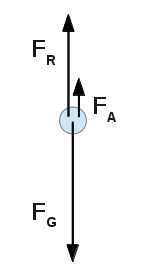
\includegraphics[width=0.24\textwidth]{MillikanMasse}
	\caption{Kräftebeziehungen beim Fall des Öltröpfchens}
	\label{fig:MillikanMasse}
\end{figure}


Setzt man die entsprechenden Teilgleichungen (Gewichtskraft einer Kugel $F_G = V \rho g = \frac{4}{3} \pi r^3 \rho_{O} g$ und Auftrieb einer Kugel in der Luft $F_A = V \rho g = \frac{4}{3} \pi r^3 \rho_L g$) ein, erhält man für $r$:

\begin{align} \label{eq:StokesReibungFuerR}
\begin{split}
	F_R &= F_G - F_A \\
	6 \pi \eta v_O r &= \frac{4}{3} r^3 \pi \rho_{O} g - \frac{4}{3} r^3 \pi \rho_{L} g \\
	r &= \sqrt{\frac{9v_{O}\eta}{2(\rho_{O}-\rho_{L}) \cdot g}}
\end{split}
\end{align}

Hierbei ist $v_{0}$ besagte Fallgeschwindigkeit, $\eta$ (sprich: \glqq klein Eta\grqq) die Viskosität der Luft, $\rho$ (sprich: \glqq klein Rho\grqq) jeweils die Dichte des Öls ($\rho_O$), respektive von Luft ($\rho_L$) und $g$ die Fallbeschleunigung.

Da man nun den Radius $r$ bestimmen kann, kann man auch das Volumen und dann, über die Dichte, auch die Masse des Ölkörpers berechnen:


\subsection{Bestimmung von $q$}

Die eigentlich Bestimmung von $q$ ergibt sich aus dem Gleichsetzen von $F_{el}$ und $F_G$, wie schon angesprochen. Allerdings muss hier auch noch die Auftriebskraft $F_A$ in der Luft mit eingerechnet werden, welche in der gegebenen Größenordnung nicht zu vernachlässigen ist.

Anstelle von $F_{el} = F_G$ ergibt sich:

\begin{align}
\begin{split}
	F_{el} &= F_G - F_A \\
	\frac{qU}{d} &= \frac{4}{3} \pi r^3 \rho_{O} g - \frac{4}{3} \pi r^3\rho_{L} g \\
	\frac{qU}{d} &= \frac{4}{3} \pi  r^3(\rho_{O} - \rho_{L}) g \\
	q &= \frac{d}{U} \cdot \frac{4}{3} \pi r^3 (\rho_{O} - \rho_{L}) g \\
\end{split}
\end{align}

\noindent Jetzt noch den Radius $r$ von der Stokesreibung einsetzten:

\begin{align}
\begin{split}
	q &= \frac{d}{U} \cdot \frac{4}{3} \pi \sqrt{\frac{9v_{O}\eta}{2(\rho_{O}-\rho_{L}) \cdot g}}^3 (\rho_{O} - \rho_{L}) g \\
	q &= \frac{d}{U} \cdot 9\sqrt{2} \pi \cdot \sqrt{\frac{v_{O}^3 \cdot \eta^3}{(\rho_O - \rho_L) \cdot g}}
\end{split}
\end{align}

Damit existiert eine Gleichung für die Ladung $q$ eines Öltröpfchen, die nur aus messbaren Größen besteht.

\begin{Anmerkung}
Natürlich kann und muss die Herleitung als Schüler nicht komplett nachvollzogen werden. Wichtig sind ist der Ansatz und das Auftreten des Masseproblems. Wie genau dieses gelöst würde, ist nicht von unabdingbarer Bedeutung. Das Curriculum legt den Fokus mehr auf die richtige Interpretation der Ergebnisse; beschrieben im nächsten Abschnitt.
\end{Anmerkung}


\subsection{Ergebnisse}

\begin{figure}[h!]
	\center
	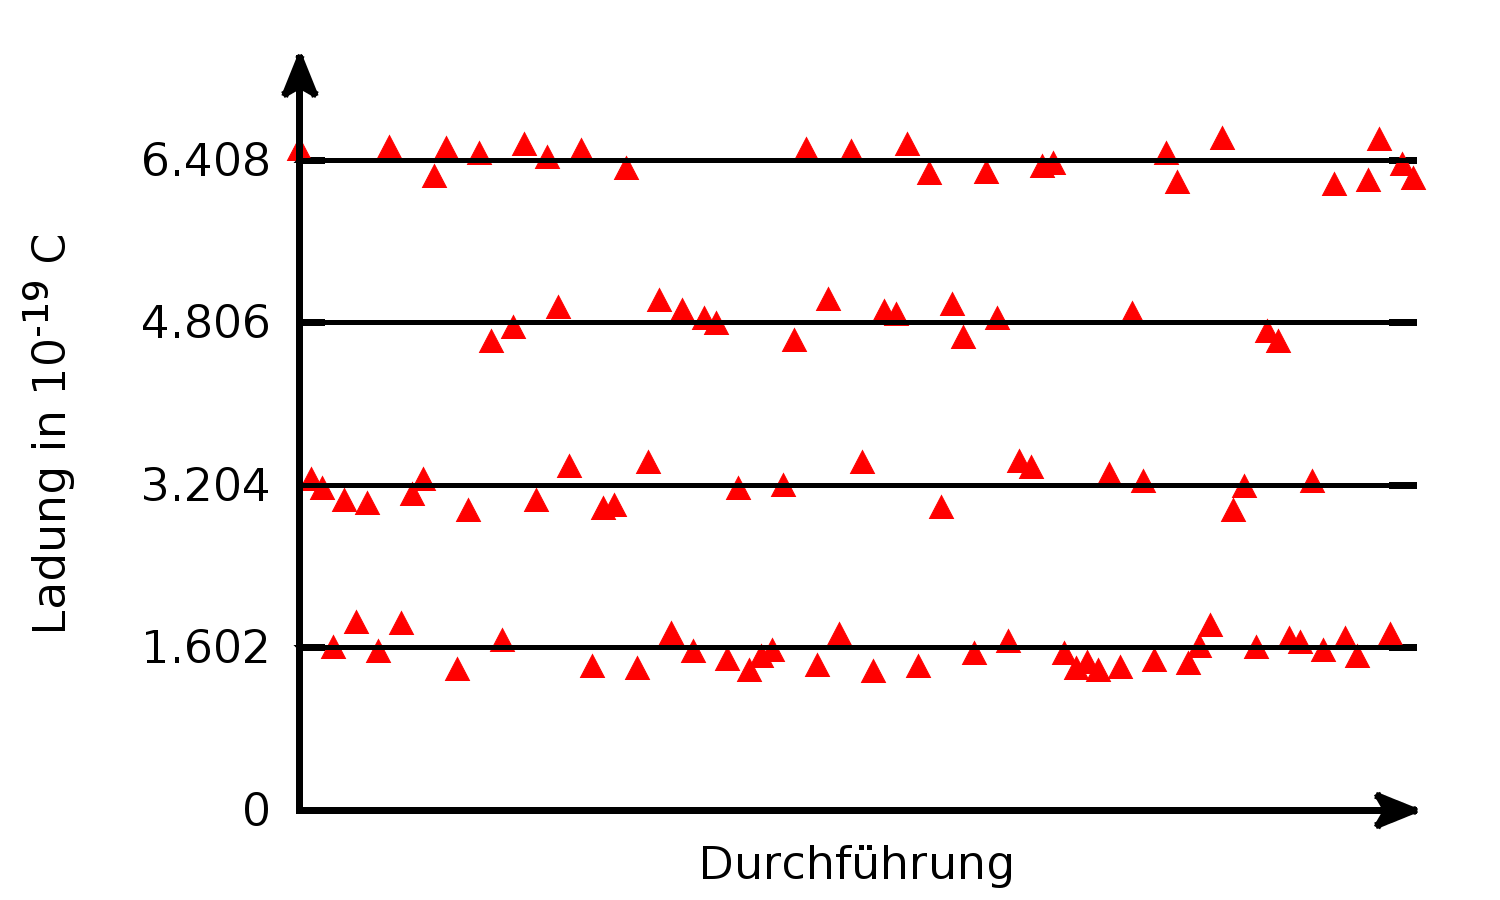
\includegraphics[width=0.8\textwidth]{plot_Millikan_Auswertung}
	\begin{comment}
Gnuplot: './plot_millikan.p'
	\end{comment}
	\caption{Auswertung via Graph: Ladung über der Nummer der  Durchführung}
	\label{fig:millikan_auswertung}
\end{figure}

Wenn man die Ergebnisse wie in Grafik \ref{fig:millikan_auswertung}\endnote{\glqq Millikan Beispielwerte\grqq{} von Till Blaha - Eigenes Werk. Lizenziert unter Gemeinfrei.} aufführt, fällt auf, dass sich eine sogenannte Quantisierung einstellt. Das heißt, dass die Ladung nicht \glqq Stufenlos\grqq{} sondern in \glqq Sprüngen\grqq{} existiert. Mathematisch heißt das, dass die Ladungen der Tröpfchen Vielfache einer kleinsten Einheit sind, Vielfache der \glqq Elementarladung\grqq .

Diese Elementarladung (in Coulomb $C$) mit Formelzeichen $q_e$ oder $e$ (seltener auch einfach $q$, wobei Verwechslungsgefahr mit der generellen Ladung eines Körpers, ebenfalls $q$, besteht) wurde von den Forschern als Ladung eines einzelnen Elektrons interpretiert\endnote{Phrase von: \url{https://nl.wikipedia.org/wiki/Proef_van_Millikan}}. Auf dem Casio fx991xx Taschenrechner existiert die Konstante Nr. 23:

\begin{align}
	q_e \approx 1,602 \cdot 10^{-19} C
\end{align}

Alle Ladungen, die uns begegnen sind also Vielfache dieser Elementarladung. Dies war eine ziemlich bahnbrechende Entdeckung, die Millikan schließlich auch den Nobelpreis einbrachte. Man kann mit ihr z.B. berechnen, wie groß der Überschuss an Elektronen über Protonen auf einem Körper ist, wenn man dessen Ladung kennt:

\begin{align}
	n_{ueberschuss} = \frac{q}{q_e}
\end{align}


\subsection{Applet}

Es gibt online eine Vielzahl Applets\endnote{Millikanversuch als Applet: \url{http://ne.lo-net2.de/selbstlernmaterial/p/e/mi/java1/mi_java1.html}} mit denen man selbst den Versuch durchführen kann, empfohlene Werte für die Dichten und Viskositäten sind ebenfalls auf genannter Website zu finden.




